\section{Cadre idéal}

\subsection{Définition du cadre idéal}
Notre algorithme fonctionne parfaitement dans le cadre idéal, une fois sortie de ce cadre les résultats sont moins précis et peuvent être incohérents. \\Ayant choisi un espace de couleur RGB, le moindre changement de luminosité nous donne des résultats in cohérents. \\\\
Il faut que l'appareil tel que la webcam ou le smartphone ne bouge pas lors de la collecte des données. Si celui-ci bouge de trop nous allons détecter des variations et notre application la percevra comme des fréquneces cardiaques.\\\\
L'appareil doit enregistrer les données avec une résolution supérieure à 480*320.\\
La personne filmée ne doit être pas trop éloignée de l'objectif pour avoir des résultats optimaux.

\subsection{Résultats dans le cadre idéal}
Nous avons effectué différents tests durant le projet. En utilisant les vidéos fournies sur le site dû MIT\@. Notre logiciel arrive à obtenir des 
résultats très correct. En effet, par exemple comme on peut le voir sur cette capture d'écran. Après notre magnification réalisée, on retrouve
une fréquence cardiaque d'environ 53 battements par minute (BPM), l'article du MIT lui trouve une fréquence de 54 BPM\@. 

\begin{figure}[h!]
	\centering
	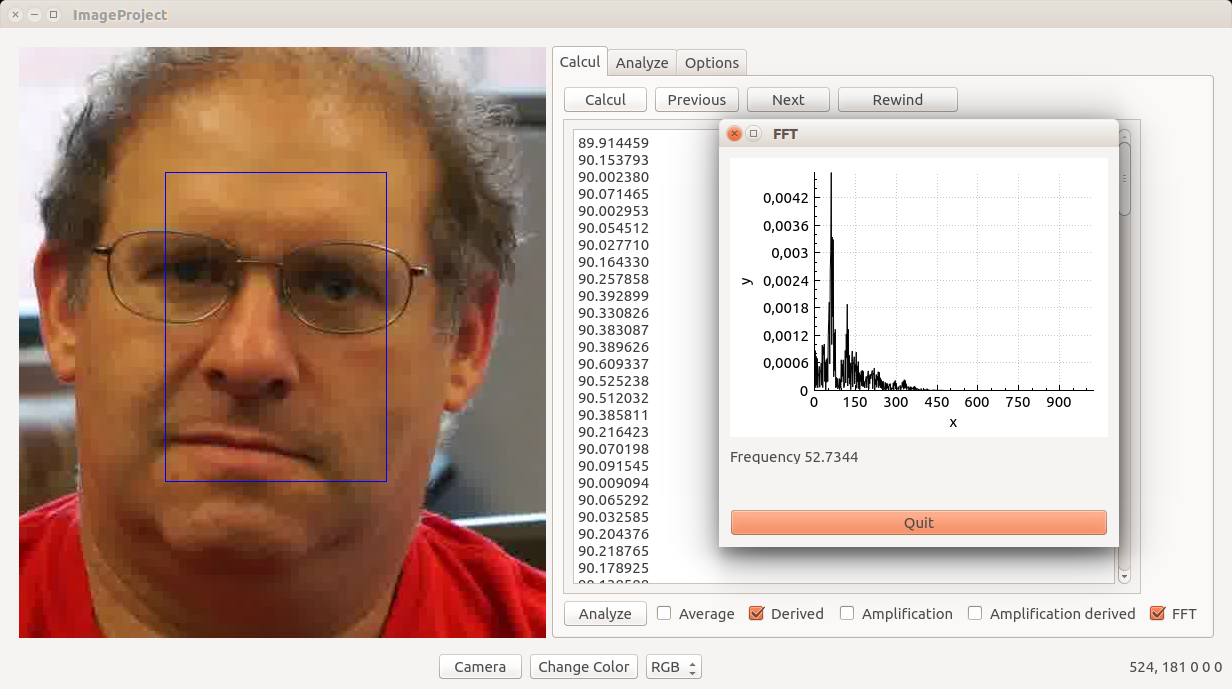
\includegraphics[width=0.9\textwidth]{data/cas-ideal.png}
	\caption{Vidéo source du MIT analysé avec notre logiciel.}
\end{figure}

On pouvait se poser la question, des personnes de couleur, est-ce qu'une couleur de peau différente aurait pu avoir des conséquences? Nous avons
donc tester avec une autre vidéo fournie par le MIT avec une personne de peau noir, on peut voir sur la capture suivante que cela n'a en rien influencer
sur notre algorithme. On retrouve donc une fréquence comprise entre 47 et 59 BPM\@.

\begin{figure}[h!]
	\centering
	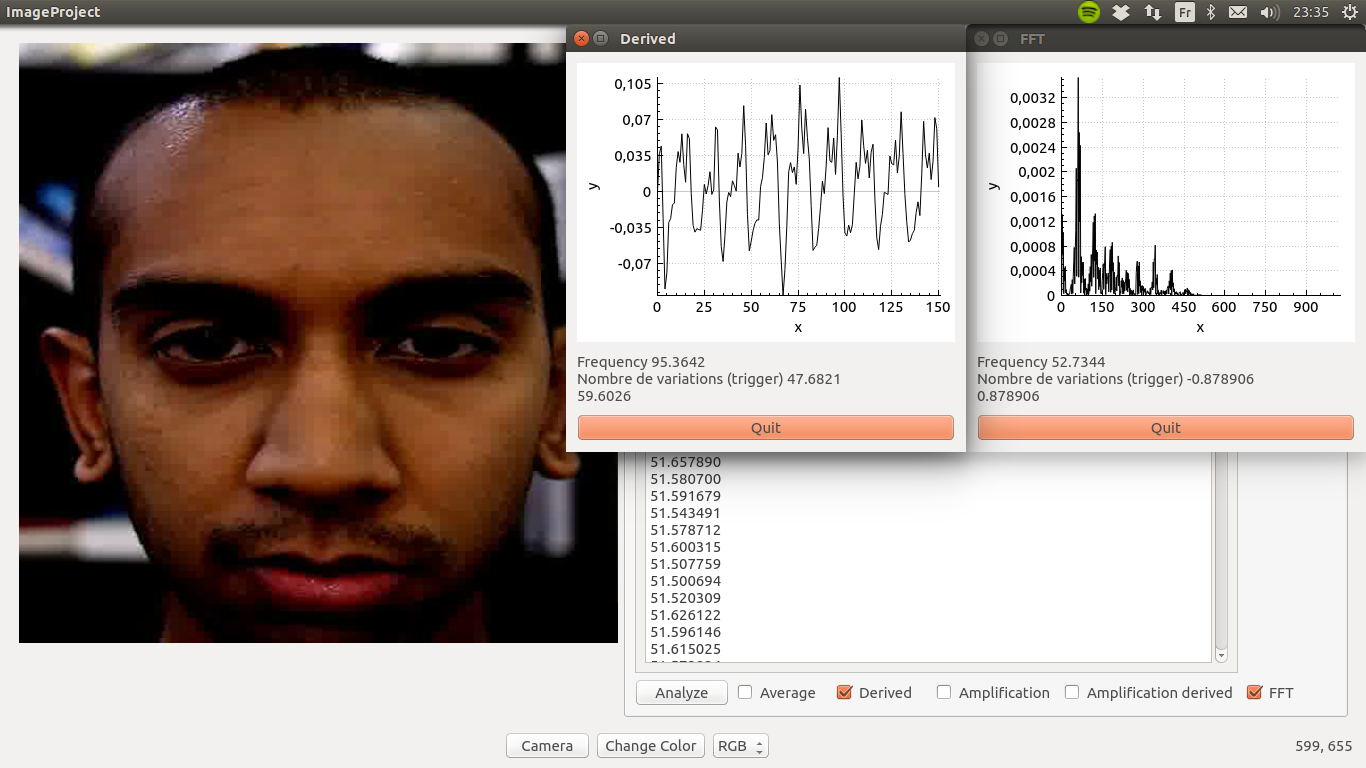
\includegraphics[width=0.9\textwidth]{data/logi.png}
	\caption{Autres test avec une personne de couleur de peau différente.}
\end{figure}


\section{Webcam}

Avec une webcam, nos résultats sont moins précis, mais sont assez correct pour être utiliser. 

\begin{figure}[h!]
	\centering
	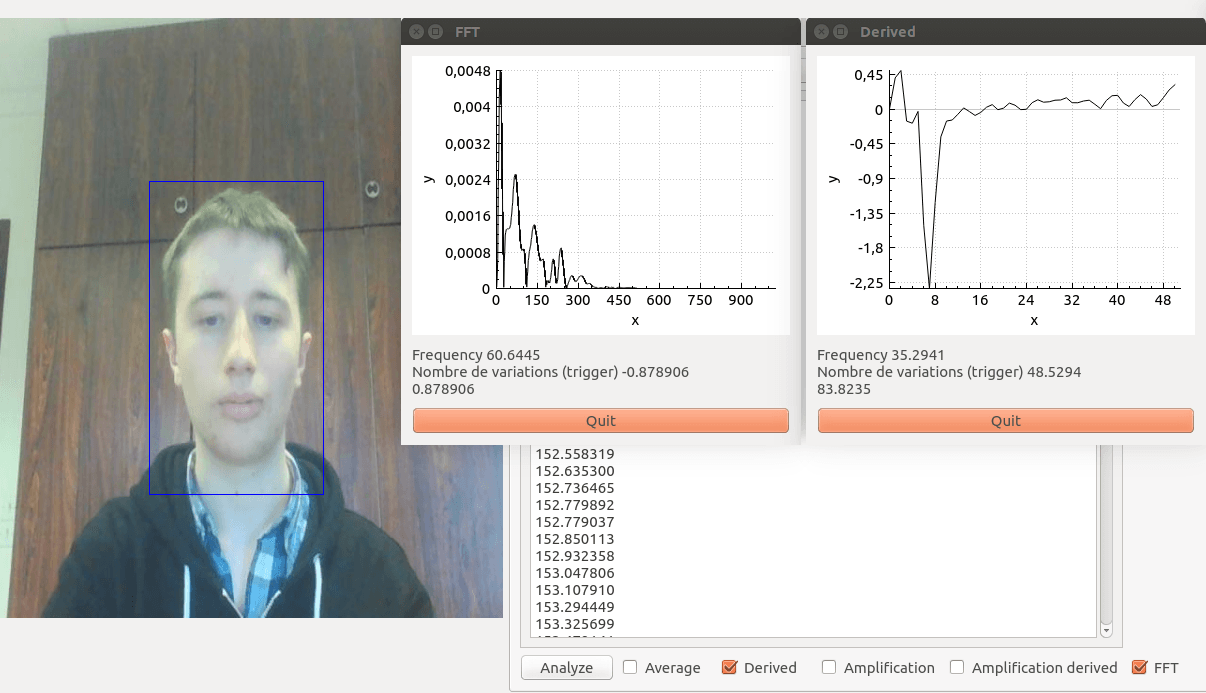
\includegraphics[width=1\textwidth]{data/webcam.png}
	\caption{Vidéo pris par la webcam et analysé avec notre logiciel.}
\end{figure}

\section{Mobile}

\subsection{Android}

Notre plus gros problème a était lors de nos tests sur Android, la stabilité de la vidéo et le nombre de frames capturés.
Actuellement notre application est capable de capturer des frames et appliquer notre algorithme mais nos résultats restent erronées.

\subsection{OpenCV}
L'utilisation d'une FFT et d'un Trigger permet de mieux différencier l'homme de la photo. Même si les résultats sont meilleurs il reste de nombreuses erreurs et le temps de calcul est beaucoup plus long.

\subsection{Ressources utilisées}
La mémoire accordé à notre application par le système d'exploitation de l'ordinateur est fixe et ne peut être augmenté.\\
Donc nous devons faire nos enregistements avec une mémoire limitée, c'est à dire que le nombre d'image capturée était limité. Une plus grand resolution de la caméra implique donc moins d'images à enregistrer. \\
De plus le nombre d'opération a effectué étant important, nous avions un temps de calcul assez important sous OpenCV\@. Pour 10 secondes d'enregistement avec une résolution de 480*320 à raison de 6 images par seconde, soit 60 images nous obtenions un temps de calcul de 20 secondes. Ce qui es beaucoup trop important pour une application qui se veut rapide.\\
Sous android natif le problème fut que le nombre d'images capturé n'était pas suffisant pour permettre une analyse correcte, un enregistement d'un nombre trop important d'image (supérieur à 30) engendrait un crash de notre application.



\section{Bilan}

Notre différenciation entre un humain et une photo fonctionne correctement dès lors où la stabilité est assurée. En effet, prenons Android, nous arrivons
à capturer plus de frames qu'en utilisant OpenCV, toutefois le tracking d'OpenCV est plus efficace. De ce fait, malgré une meilleure capture sous Android 
comme la stabilité est plus mauvaise, nos résultats sont moins bons. Mais à contrario, lorsqu'on utilise l'application réalisée avec OpenCV, le nombre d'images
capturé est seulement de 20 pour 4 secondes, avec si peu d'images à traiter notre magnification n'est pas correcte. C'est seulement au bout de 10 secondes
lorsqu'on capture entre 50 à 70 frames qu'on a des résultats cohérents. 

